\documentclass[12pt]{article}
\usepackage{times} 			% use Times New Roman font

\usepackage[margin=1in]{geometry}   % sets 1 inch margins on all sides
\usepackage{hyperref}               % for URL formatting
\usepackage[pdftex]{graphicx}       % So includegraphics will work
\setlength{\parskip}{1em}           % skip 1em between paragraphs
\usepackage{indentfirst}            % indent the first line of each paragraph
\usepackage{datetime}
\usepackage[small, bf]{caption}
\usepackage{listings}               % for code listings
\usepackage{xcolor}                 % for styling code
\usepackage{multirow}

%New colors defined below
\definecolor{backcolour}{RGB}{246, 246, 246}   % 0xF6, 0xF6, 0xF6
\definecolor{codegreen}{RGB}{16, 124, 2}       % 0x10, 0x7C, 0x02
\definecolor{codepurple}{RGB}{170, 0, 217}     % 0xAA, 0x00, 0xD9
\definecolor{codered}{RGB}{154, 0, 18}         % 0x9A, 0x00, 0x12

%Code listing style named "gcolabstyle" - matches Google Colab
\lstdefinestyle{gcolabstyle}{
  basicstyle=\ttfamily\small,
  backgroundcolor=\color{backcolour},   
  commentstyle=\itshape\color{codegreen},
  keywordstyle=\color{codepurple},
  stringstyle=\color{codered},
  numberstyle=\ttfamily\footnotesize\color{darkgray}, 
  breakatwhitespace=false,         
  breaklines=true,                 
  captionpos=b,                    
  keepspaces=true,                 
  numbers=left,                    
  numbersep=5pt,                  
  showspaces=false,                
  showstringspaces=false,
  showtabs=false,                  
  tabsize=2
}

\lstset{style=gcolabstyle}      %set gcolabstyle code listing

% to make long URIs break nicely
\makeatletter
\g@addto@macro{\UrlBreaks}{\UrlOrds}
\makeatother

% for fancy page headings
\usepackage{fancyhdr}
\setlength{\headheight}{13.6pt} % to remove fancyhdr warning
\pagestyle{fancy}
\fancyhf{}
\rhead{\small \thepage}
\lhead{\small HW 1\, Venkatesh}  % EDIT THIS, REPLACE # with HW number
\chead{\small CS 532, Fall 2021} 

%-------------------------------------------------------------------------
\begin{document}

% EDIT THE ITEMS HERE
\begin{centering}
{\large\textbf{HW 1\ - Web Science Intro}}\\ 
Swathi Venkatesh\\
09/18/2021\\
\end{centering}

%-------------------------------------------------------------------------

% The * after \section just says to not number the sections
\section*{Q1}

\emph{Consider the "bow-tie" structure of the web in the Broder et al. paper "Graph Structure in the Web" that was described in Module 1.
}
\emph{Now consider the following links:}


\emph{Draw the resulting directed graph (either sketch on paper or use another tool) showing how the nodes are connected to each other and include an image in your report. This does not need to fit into the bow-tie type diagram, but should look more similar to the graph on slide 24 from Module-01 Web-Science-Architecture.}
\newline
A -> B\newline
B --> C\newline
B --> D\newline
C --> A\newline
C --> E\newline
E --> C\newline
E --> G\newline
F --> E\newline
H --> G\newline
I --> A\newline
I --> M\newline
I --> N\newline
J --> K\newline
L --> D\newline
M --> D\newline
\newline
\emph{For the graph, list the nodes (in alphabetical order) that are each of the following categories:}
•	SCC:\newline
•	IN:\newline
•	OUT:\newline
•	Tendrils:\newline
      o	indicate if the tendril is reachable from IN or can reach OUT\newline
•	Tubes:\newline
      o	explain how the nodes serve as tubes\newline
•	Disconnected:


\subsection*{Answer}


Figure 1 shows the Bow-tie structure of the given link.

\begin{figure}[h]
    \centering
    % trim and clip are used to crop the image, trim=left bottom right top
    % width sets max width, height will be scaled appropriately
    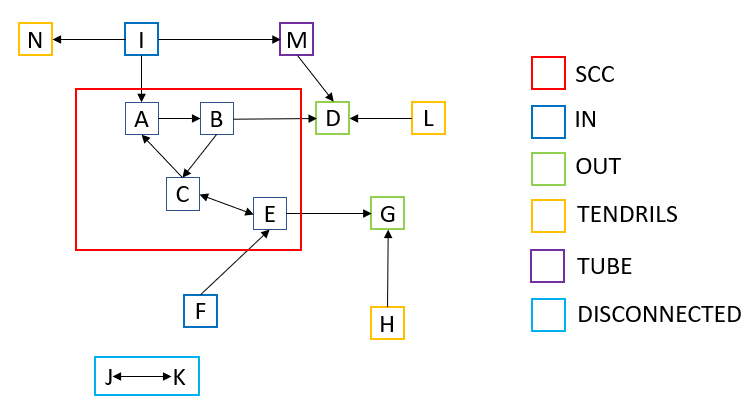
\includegraphics[trim=0 0 10 8, clip, width=\textwidth] {one1.PNG}
    \caption{Bow-tie structure of the given link}
    \label{fig:web-growth}
\end{figure}
SCC: It stands for strongly connected network.  In the Figure 1 the nodes A, B, C, E are connected to one another. They are belong to one SCC.
\newline
\newline
IN: In the Figure 1 nodes I and F belong to IN category because they can reach the SCC but can’t be reached by it.
\newline
\newline
OUT: In the Figure 1 nodes D and G belong to OUT category. They are nodes that can be reached from SCC but they don't link back to it.
\newline
\newline
Tendrils: In the Figure 1 the nodes  N, L, H  and M belong to tendrils. The tendril comes from the IN group (node I and M) and into the outgroup (node D and G). These nodes cannot reach the SCC and also cannot be reached by the SCC.
\newline
\newline
Tubes: In the Figure 1 the node M belong to tube as it connects IN node to OUT node by temporary routing the SCC. Node M has inlink from the node I (IN group) and has outlink to node D (OUT group) without crossing SCC.
\newline
\newline
Disconnected: In the Figure 1 the node J and K are disconnected as they have no inlink from other nodes and no outlink to other nodes.



\subsection*{Discussion}

The tools such as Microsoft Power Point was used to create the Figure 1.

\section*{Q2}
Demonstrate that you know how to use curl and are familiar with the available options.
\newline
\newline
URI to request: \url{http://www.cs.odu.edu/~mweigle/courses/cs532/ua_echo.php}

a) First, load the URI directly in your browser and take a screenshot. The resulting webpage should show the "User-Agent" HTTP request header that your web browser sends to the web server.
\newline
\newline
b) In a single curl command, request the URI, show the HTTP response headers, follow any redirects, and change the User-Agent HTTP request field to "CS432/532". Show command you used and the result of your execution on the command line. (Either take a screenshot of your terminal or copy/paste into a code segment.)
\newline
\newline
c) In a single curl command, request the URI, follow any redirects, change the User-Agent HTTP request field to "CS432/532", and save the HTML output to a file. Show the command you used and the result of your execution on the command line. View the HTML output file that was produced by curl in a web browser and take a screenshot.
\newline
\newline
Explain the results you get for each of these steps.

\subsection*{Answer}

a) The Figure 2 shows the User-Agent HTTP header that the browser sends to the web server.
\newline
Figure 2 shows the URI opened in the browser.

\begin{figure}[h]
    \centering
    % trim and clip are used to crop the image, trim=left bottom right top
    % width sets max width, height will be scaled appropriately
    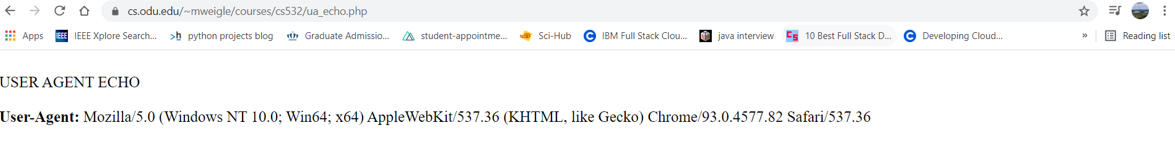
\includegraphics[trim=0 0 10 8, clip, width=\textwidth] {two.PNG}
    \caption{URI opened in the browser}
    \label{fig:web-growth}
\end{figure}
\newline
\newline
b) The curl command used here is:
\newline\newline
curl -v -L -H "User-Agent: CS432/532"  http://www.cs.odu.edu/~mweigle/courses/cs532/ua_echo.php
\newline

The –v stands for verbose. This option is used to get more data on the input. In the curl command above all the details about the user agent are displayed because of –v option.

-L: this option is used when the request made has been moved to another location. In the output we can see that the web link has 301 status that means redirection has taken place and requested page is moved to different location.

-H: the header content is changed using the –H option. In the above command the user agent is set to CS432/532 because of the –H option.

After executing the above command the User-Agent is displayed as CS 432/532. The screenshot provides the result of execution of the above command.
\begin{figure}[h]
    \centering
    % trim and clip are used to crop the image, trim=left bottom right top
    % width sets max width, height will be scaled appropriately
    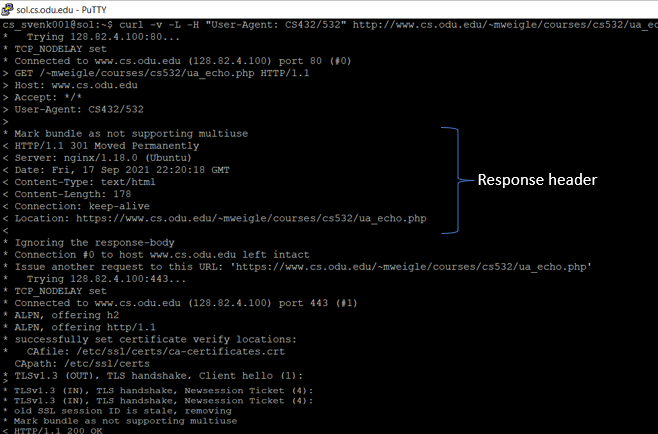
\includegraphics[trim=0 0 0 0, clip, width=\textwidth] {thre.PNG}
    \caption{Code executed using curl command}
    \label{fig:web-growth}
\end{figure}
\newline
\newline
\newline
c) The curl command used here is:\newline
curl -o "one.html" -v -H "User-Agent:CS432/532" http://www.cs.odu.edu/~mweigle/courses/cs532/ua_echo.php 

-o: this option is used to save the curl output to the file.

-L: this option is used when the request made has been moved to another location. In the output we can see that the web link has 301 status that means redirection has taken place and requested page is moved to different location.

-H: the header content is changed using the –H option. In the above command the user agent is set to CS432/532 because of the –H option.

Figure 4 shows the command used to change User-Agent to CS432/532 and Figure 5 shows the output in web browser when User-Agent is changed to CS432/532.

\begin{figure}[h]
    \centering
    % trim and clip are used to crop the image, trim=left bottom right top
    % width sets max width, height will be scaled appropriately
    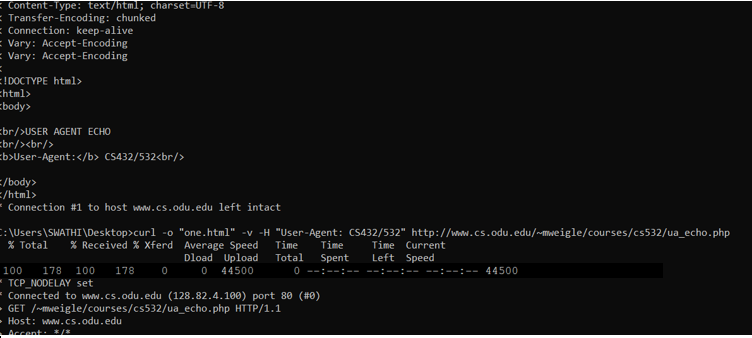
\includegraphics[trim=0 0 10 8, clip, width=\textwidth] {jj.PNG}
    \caption{User agent output in command line}
    \label{fig:web-growth}
\end{figure}
\newline
\begin{figure}[h]
    \centering
    % trim and clip are used to crop the image, trim=left bottom right top
    % width sets max width, height will be scaled appropriately
    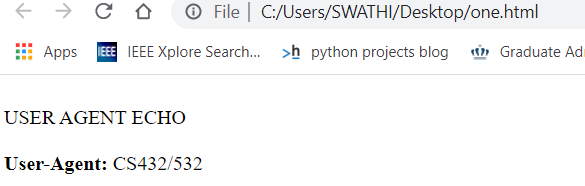
\includegraphics[trim=0 0 10 8, clip, width=\textwidth] {jj2.PNG}
    \caption{User agent output in web browser}
    \label{fig:web-growth}
\end{figure}
\subsection*{Discussion}
The curl documentation and slides were referred to work on it.
\section*{Q3}
Write a Python program to find links to PDFs in a webpage.

Your program must do the following:

take the URI of a webpage as a command-line argument
extract all the links from the page
for each link, request the URI and use the Content-Type HTTP response header to determine if the link references a PDF file
for all links that reference a PDF file, print the original URI (found in the source of the original HTML), the final URI (after any redirects), and the number of bytes in the PDF file. (Hint: Content-Length HTTP response header)
Here is a snippet of the expected operation:

Show that the program works on 3 different URIs, one of which must be https://www.cs.odu.edu/~mweigle/courses/cs532/pdfs.html, which contains 8 links to PDFs.

Many faculty members have a list of their publications in PDF form on their webpages. You can discover ODU CS faculty webpages is through the Research page on the CS homepage. Click on a faculty member's name and that will take you to their ODU directory page. Most of us have another link on that page that goes to our homepages where you can then find a list of publications that will often link to PDFs.\newline\newline
Also, there are a set of pages linked on our CS 432/532 Syllabus that say "pdf available". If you follow some of those links, you'll likely find a page that links to at least one PDF.\newline\newline
You will likely want to use the BeautifulSoup Python library for this question. On the ODU-CS Linux machines, you may need to run pip3 install beautifulsoup4 before you can use BeautifulSoup, but you don't need root privileges to do this.
\subsection*{Answer}
%Python code highlighting
\begin{lstlisting}[language=Python, caption=Python code, label=lst:copy]
import sys
from bs4 import BeautifulSoup
import requests
if __name__ == '__main__':
    u = sys.argv[1]
pt = 'application/pdf'
if u != '':
    file = requests.get(u)
        # getting html file from response
    html = file.text

    for link in BeautifulSoup(html, 'html.parser').find_all('a', attrs={'href': True}):
        file = requests.get(link['href'])
        o = file.url
        i = 0
        for url in file.history:
            i+= 1
            if i > 100:
                break
            continue
            # fetch final url after checking if it is pdf link or not
        f = file.url
            # examine if content type is pdf link
        if file.headers['Content-Type'] == pt:
            cl = file.headers['Content-Length']
            print(f'Original URL: {o}\n'f'Final URL: {f}\n'f'ContentLength: {cl} bytes\n')
else:print('')


\end{lstlisting}
\newline

%Python code highlighting
\begin{lstlisting}[language=Python, caption=Python code, label=lst:copy]
C:\Users\SWATHI\PycharmProjects\bnm>python api.py https://www.cs.odu.edu/~mweigle/courses/cs532/pdfs.html
Original URL: https://www.cs.odu.edu/~mln/pubs/ht-2018/hypertext-2018-nwala-bootstrapping.pdf
Final URL: https://www.cs.odu.edu/~mln/pubs/ht-2018/hypertext-2018-nwala-bootstrapping.pdf
ContentLength: 994153 bytes

Original URL: https://www.cs.odu.edu/~mln/pubs/ipres-2018/ipres-2018-atkins-news-similarity.pdf
Final URL: https://www.cs.odu.edu/~mln/pubs/ipres-2018/ipres-2018-atkins-news-similarity.pdf
ContentLength: 18995885 bytes

Original URL: https://www.cs.odu.edu/~mln/pubs/ipres-2018/ipres-2018-jones-off-topic.pdf
Final URL: https://www.cs.odu.edu/~mln/pubs/ipres-2018/ipres-2018-jones-off-topic.pdf
ContentLength: 3119205 bytes

Original URL: https://www.cs.odu.edu/~mln/pubs/ipres-2018/ipres-2018-jones-archiveit.pdf
Final URL: https://www.cs.odu.edu/~mln/pubs/ipres-2018/ipres-2018-jones-archiveit.pdf
ContentLength: 2639215 bytes

Original URL: https://www.cs.odu.edu/~mln/pubs/jcdl-2018/jcdl-2018-nwala-scraping-serps-seeds.pdf
Final URL: https://www.cs.odu.edu/~mln/pubs/jcdl-2018/jcdl-2018-nwala-scraping-serps-seeds.pdf
ContentLength: 2172494 bytes

Original URL: https://www.cs.odu.edu/~mln/pubs/jcdl-2018/jcdl-2018-kelly-private-public-web-archives.pdf
Final URL: https://www.cs.odu.edu/~mln/pubs/jcdl-2018/jcdl-2018-kelly-private-public-web-archives.pdf
ContentLength: 2553579 bytes

Original URL: https://www.cs.odu.edu/~mln/pubs/jcdl-2018/jcdl-2018-aturban-archivenow.pdf
Final URL: https://www.cs.odu.edu/~mln/pubs/jcdl-2018/jcdl-2018-aturban-archivenow.pdf
ContentLength: 3998654 bytes

Original URL: https://www.cs.odu.edu/~mln/pubs/jcdl-2018/jcdl-2018-alam-archive-banner.pdf
Final URL: https://www.cs.odu.edu/~mln/pubs/jcdl-2018/jcdl-2018-alam-archive-banner.pdf
ContentLength: 596000 bytes




\end{lstlisting}

\begin{figure}[h]
    \centering
    % trim and clip are used to crop the image, trim=left bottom right top
    % width sets max width, height will be scaled appropriately
    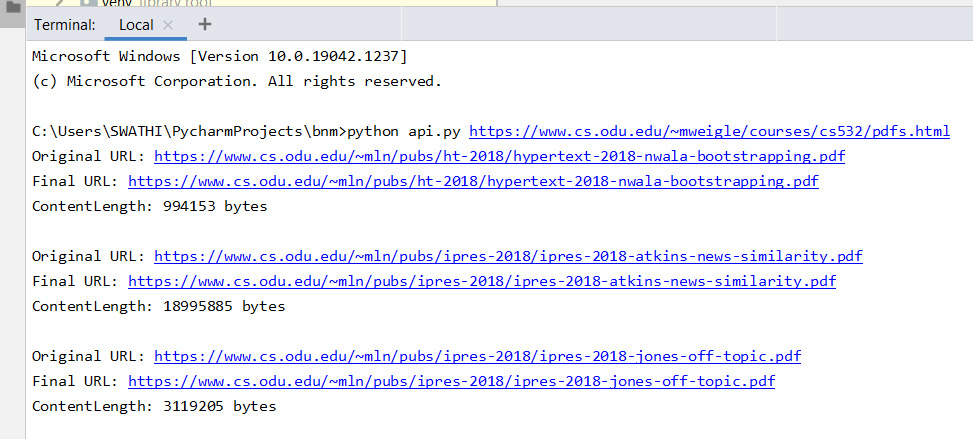
\includegraphics[trim=0 0 10 8, clip, width=\textwidth] {si.PNG}
    \caption{Program output}
    \label{fig:web-growth}
\end{figure}

\begin{figure}[h]
    \centering
    % trim and clip are used to crop the image, trim=left bottom right top
    % width sets max width, height will be scaled appropriately
    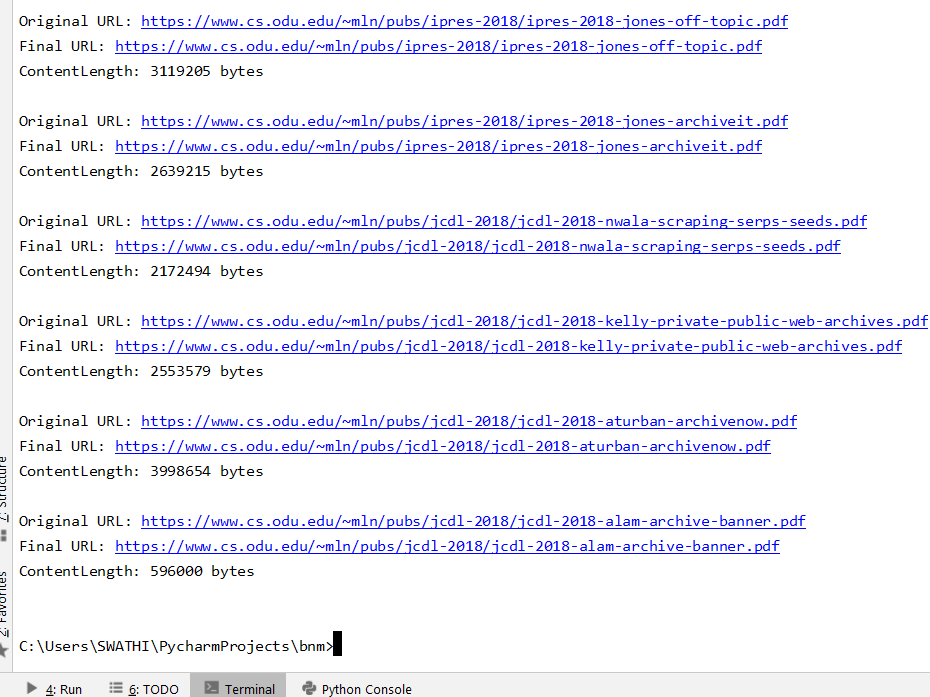
\includegraphics[trim=0 0 10 8, clip, width=\textwidth] {si1.PNG}
    \caption{Program output}
    \label{fig:web-growth}
\end{figure}
\subsection*{Discussion}
The Pycharm 2019.2.3 is used to execute the code.
\section*{References}



\begin{itemize}
    \item {CodeGrepper, \url{https://www.codegrepper.com/code-examples/python/how+to+find+pdf+file+in+link+beautifulsoup}}
    \item {Use of BeautifulSoup, \url{https://www.dataquest.io/blog/web-scraping-python-using-beautiful-soup/}}
    \item {Github , \url{https://github.com}}
    \item {StackOverFlow , \url{https://stackoverflow.com/questions/866946/how-can-i-see-the-request-headers-made-by-curl-when-sending-a-request-to-the-ser}}
    \item {Curl Usage , \url{https://mkyong.com/web/curl-display-request-headers-and-response-headers/}}
    \item {Curl documentation , \url{https://stackoverflow.com/questions/21226980/curl-output-to-file}}
\end{itemize}

\end{document}

